Essa etapa envolveu a implementação do DPD em FPGA, o que exige a paralelização das operações aritméticas. Em cada ciclo de clock, três operações são realizadas simultaneamente: o sinal atual é elevado ao quadrado, armazenado em um registrador de deslocamento dentro de uma matriz de extração \footnote{matriz que contém todas as potências e amostras anteriores necessárias para o cálculo da saída}, o cálculo do produto de todos os elementos da matriz de extração e a soma dos produtos entre os sinais do mesmo instante e seus respectivos coeficientes. Esse processo se repete \( P \) vezes, correspondendo ao grau \( P \) do polinômio de memória. Como consequência, a saída do DPD estará incompleta durante os primeiros \( P \) ciclos de clock, pois, nesse intervalo, o cálculo depende de amostras de sinais anteriores que ainda não foram processadas, resultando em uma saída parcial.
A Figura \ref{fig:diagramaprocess} ilustra como esse processo está dividido entre cada ciclo de clock.

\begin{figure}[htbp!]
	\centering
	\captionsetup{justification=centering}
	\caption*{Fonte: Autor}
	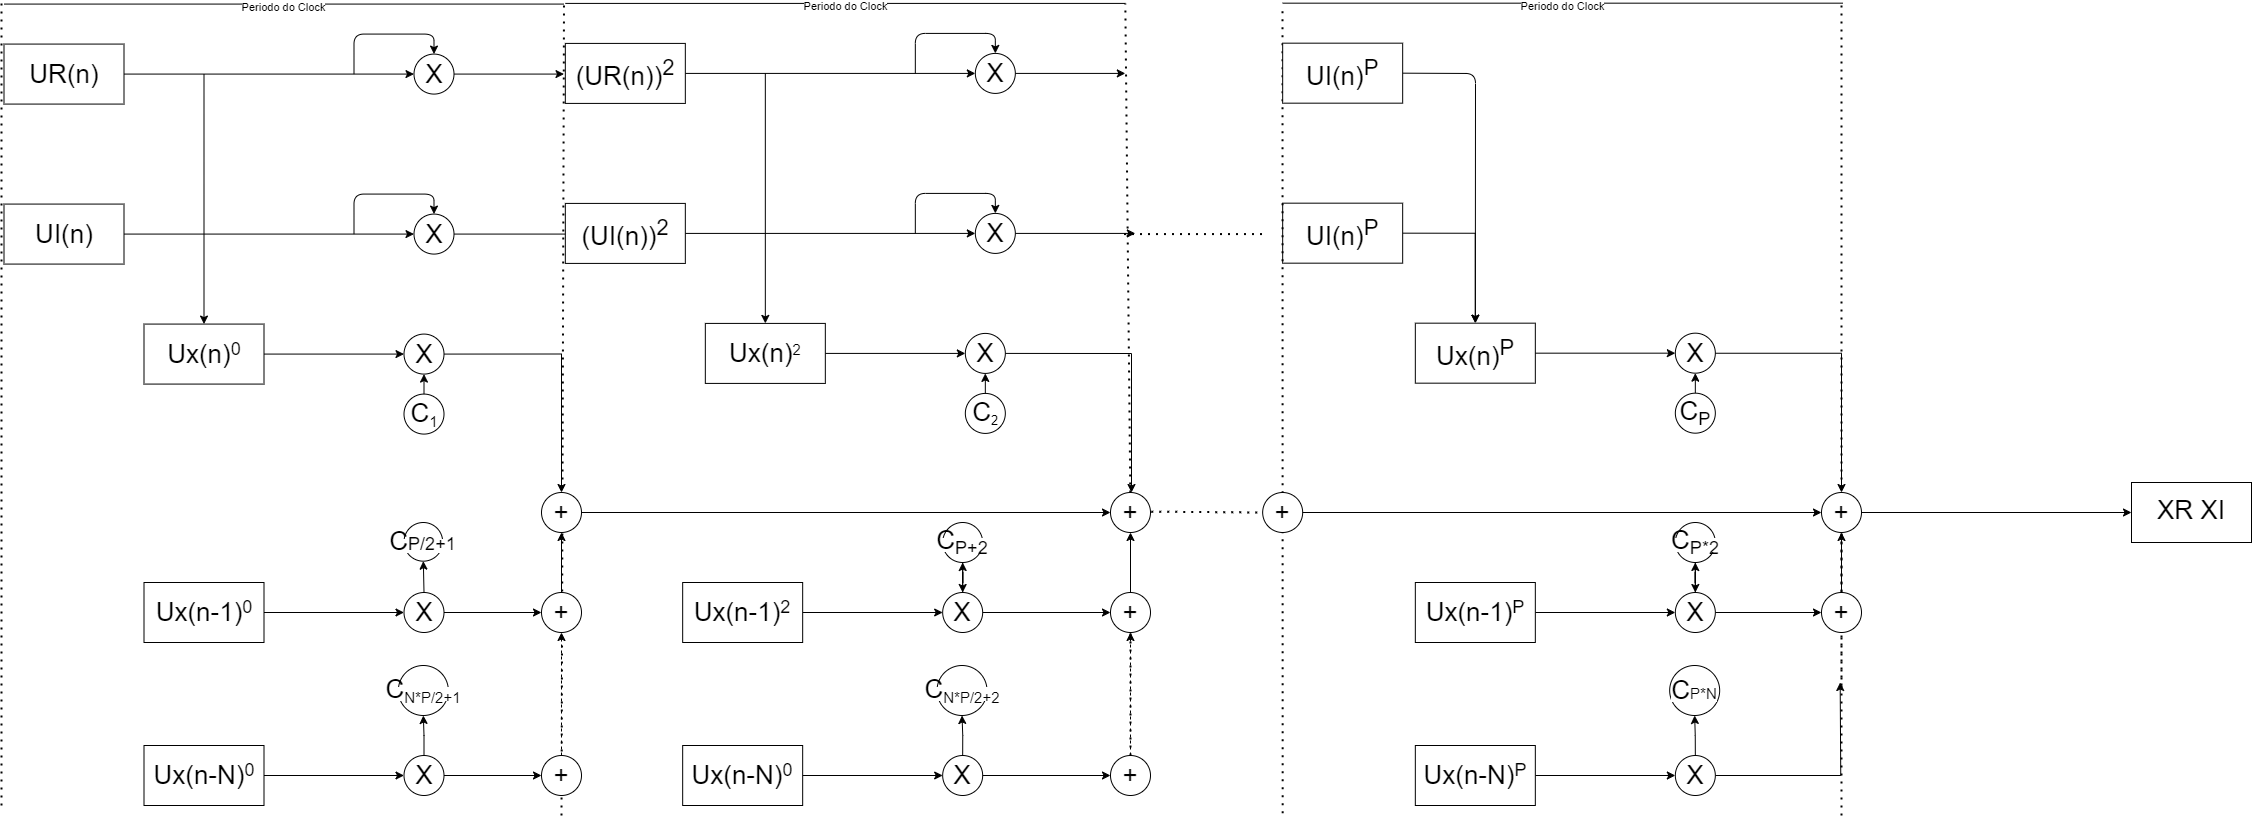
\includegraphics[width=0.50\textwidth]{diagrama_process.png}
	\caption{Processo de cálculo da saída}
	\label{fig:diagramaprocess}
\end{figure}
Conforme exibido no diagrama, cada etapa do processo fornece os dados necessários para a próxima fase do cálculo com um atraso de um ciclo de clock. Contudo, é importante destacar que o processo completo demanda ciclos adicionais, uma vez que o sinal de saída só é registrado na borda de subida seguinte do clock, garantindo a sincronização adequada no fluxo de dados.
